% ============================================================
% MAT670_46, pages 24--46.
% Pages 24--31: continuation of Lecture 5 (classification of Coxeter graphs).
% Pages 32--46: Lecture 6 (root systems -> root lattices; codes).
% ============================================================
\tikzset{L04bv/.style={circle,draw,fill=white,inner sep=0pt,minimum size=6pt},
         L04bdbl/.style={double,double distance=2pt},
         L04blab/.style={font=\scriptsize}}

\section{Classification of Coxeter graphs (continued)}
\label{L04b:sec:coxeter-cont}
\orig{continues Lecture 5 from p.~23}

Recall from the previous pages: a connected admissible diagram is a tree; each vertex
meets at most three edges counted with multiplicity; the only admissible diagram with a
triple edge is \tikz[baseline=-3pt]{\node[L04bv] (a) at (0,0) {}; \node[L04bv] (b) at (0.6,0) {};
\draw (a.north east)--(b.north west); \draw (a)--(b); \draw (a.south east)--(b.south west);}
($G_2$); and a simple chain $\{v_1,\dots,v_k\}$ may be collapsed to the single unit vector
$v=\sum_i v_i$, leaving an admissible diagram. From now on only single and double edges occur.

\subsection{Forbidden configurations}

\begin{proposition}\label{L04b:prop:forbidden}
Coxeter graphs of admissible diagrams containing any of the following subgraphs are forbidden:
\begin{center}
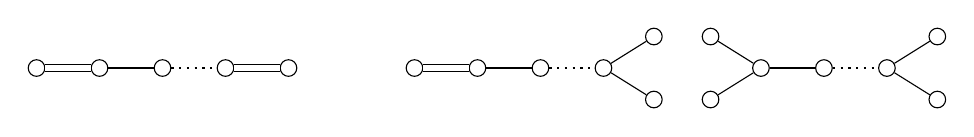
\begin{tikzpicture}[scale=0.8]
  % two double edges
  \foreach \i in {0,1,2,3,4} \node[L04bv] (a\i) at (\i,0) {};
  \draw[L04bdbl] (a0)--(a1); \draw (a1)--(a2); \draw[dotted,thick] (a2)--(a3);
  \draw[L04bdbl] (a3)--(a4);
  % double edge + fork
  \begin{scope}[xshift=6cm]
  \foreach \i in {0,1,2,3} \node[L04bv] (b\i) at (\i,0) {};
  \node[L04bv] (b4) at (3.8,0.5) {}; \node[L04bv] (b5) at (3.8,-0.5) {};
  \draw[L04bdbl] (b0)--(b1); \draw (b1)--(b2); \draw[dotted,thick] (b2)--(b3);
  \draw (b3)--(b4); \draw (b3)--(b5);
  \end{scope}
  % two forks
  \begin{scope}[xshift=11.5cm]
  \node[L04bv] (c0) at (-0.8,0.5) {}; \node[L04bv] (c1) at (-0.8,-0.5) {};
  \foreach \i in {0,1,2} \node[L04bv] (d\i) at (\i,0) {};
  \node[L04bv] (c4) at (2.8,0.5) {}; \node[L04bv] (c5) at (2.8,-0.5) {};
  \draw (c0)--(d0); \draw (c1)--(d0); \draw (d0)--(d1); \draw[dotted,thick] (d1)--(d2);
  \draw (d2)--(c4); \draw (d2)--(c5);
  \end{scope}
\end{tikzpicture}
\end{center}
Hence a connected admissible diagram (with no triple edge) contains at most one branch
point \emph{or} at most one double edge, but not both.
\end{proposition}

\begin{proof}
\added{In each case collapse the simple chain joining the two special features (possibly of
length zero) to a single vertex. By the collapsing lemma the result is again admissible, but the
new vertex meets edges of total multiplicity $2+2$, $2+1+1$, or $1+1+1+1$, i.e.\ $4$, contradicting
the bound of $3$ edges (with multiplicity) at each vertex. The same argument rules out two double
edges, two branch points, or a double edge and a branch point anywhere in the tree, since they are
always joined by a simple chain.}
\end{proof}

So, besides $G_2$, the only possible connected Coxeter graphs are:
\begin{center}
\begin{tikzpicture}[scale=0.85]
  % chain with one double edge
  \foreach \x/\n/\l in {0/u1/u_1,1/u2/u_2,2.6/up/u_p,3.6/vq/v_q,5.2/v2/v_2,6.2/v1/v_1}
     {\node[L04bv] (\n) at (\x,0) {}; \node[L04blab,below=2pt] at (\x,0) {$\l$};}
  \draw (u1)--(u2); \draw[dotted,thick] (u2)--(up); \draw[L04bdbl] (up)--(vq);
  \draw[dotted,thick] (vq)--(v2); \draw (v2)--(v1);
  % branched
  \begin{scope}[xshift=8.3cm]
  \foreach \x/\n/\l in {0/a1/u_1,1/a2/u_2,2.4/ap/u_{p-1}}
     {\node[L04bv] (\n) at (\x,0) {}; \node[L04blab,below=2pt] at (\x,0) {$\l$};}
  \node[L04bv] (x) at (3.3,0) {}; \node[L04blab,below=2pt] at (3.3,0) {$x$};
  \node[L04bv] (bq) at (4.1,0.6) {}; \node[L04blab,above=2pt] at (4.1,0.6) {$v_{q-1}$};
  \node[L04bv] (b1) at (5.5,0.6) {}; \node[L04blab,above=2pt] at (5.5,0.6) {$v_1$};
  \node[L04bv] (cr) at (4.1,-0.6) {}; \node[L04blab,below=2pt] at (4.1,-0.6) {$w_{r-1}$};
  \node[L04bv] (c1) at (5.5,-0.6) {}; \node[L04blab,below=2pt] at (5.5,-0.6) {$w_1$};
  \draw (a1)--(a2); \draw[dotted,thick] (a2)--(ap); \draw (ap)--(x);
  \draw (x)--(bq); \draw[dotted,thick] (bq)--(b1);
  \draw (x)--(cr); \draw[dotted,thick] (cr)--(c1);
  \end{scope}
\end{tikzpicture}
\end{center}
together with the simple chains \tikz[baseline=-3pt]{\foreach \i/\x in {1/0,2/0.5,3/1.3,4/1.8} \node[L04bv] (s\i) at (\x,0) {};
\draw (s1)--(s2); \draw[dotted,thick] (s2)--(s3); \draw (s3)--(s4);}, which give $A_n$.

\subsection{One double edge: \texorpdfstring{$B_n$, $C_n$, $F_4$}{Bn, Cn, F4}}

Label the diagram with one double edge as above: $u_1,\dots,u_p$, then the double edge
$u_p = v_q$, then $v_q,\dots,v_1$. Put
\[
  u=\sum_{i=1}^p i\,u_i,\qquad v=\sum_{j=1}^q j\,v_j .
\]
Since the $u_i$ form a simple chain, $2\ip{u_i}{u_{i+1}}=-1$ for $1\le i\le p-1$ and all other pairs
are orthogonal. Hence
\begin{align*}
  \ip{u}{u} &= \sum_{i=1}^p i^2\ip{u_i}{u_i} + \sum_{i<j} 2ij\,\ip{u_i}{u_j}
   = \sum_{i=1}^p i^2 + \sum_{i=1}^{p-1} i(i+1)\cdot\underbrace{2\ip{u_i}{u_{i+1}}}_{=-1}\\
  &= \sum_{i=1}^p i^2 - \sum_{i=1}^{p-1} i(i+1) = p^2 - \sum_{i=1}^{p-1} i = \frac{p(p+1)}{2},
\end{align*}
and similarly $\ip{v}{v} = q(q+1)/2$.

Since the double edge $u_p = v_q$ is the only non-orthogonal relation between the two chains,
$\ip{u}{v} = pq\,\ip{u_p}{v_q}$, and $4\ip{u_p}{v_q}^2=2$. Thus
\[
  \ip{u}{v}^2 = \frac{p^2q^2}{2}.
\]
Since $u$ and $v$ are not parallel \added{(the $u_i, v_j$ are linearly independent)}, the
Cauchy--Schwarz inequality is strict: $\ip{u}{v}^2 < \ip{u}{u}\ip{v}{v}$, i.e.
\[
  \frac{p^2q^2}{2} < \frac{p(p+1)}{2}\cdot\frac{q(q+1)}{2},
  \qquad\text{so}\qquad 2pq < (p+1)(q+1),
\]
which, for integers $p,q\ge 1$, is
\[
  \boxed{(p-1)(q-1) < 2.}
\]
Hence either $p=q=2$, which is $F_4$, or $p=1$ (or $q=1$) with the other arbitrary, which is
$B_n$ and $C_n$ \added{($n=p+q$; the Coxeter graphs of $B_n$ and $C_n$ coincide, and they are
distinguished only by the direction of the arrow in the Dynkin diagram)}.

\subsection{One branch point: \texorpdfstring{$D_n$, $E_6$, $E_7$, $E_8$}{Dn, E6, E7, E8}}

Finally, take the branched diagram above, with branch vertex $x$ and three arms
$u_1,\dots,u_{p-1}$, $v_1,\dots,v_{q-1}$, $w_1,\dots,w_{r-1}$ ($p,q,r\ge 2$), the indices
increasing towards $x$. As before put
\[
  u=\sum_{i=1}^{p-1} i\,u_i,\qquad v=\sum_{i=1}^{q-1} i\,v_i,\qquad w=\sum_{i=1}^{r-1} i\,w_i .
\]
Note that $u,v,w$ are mutually orthogonal vectors (no edges between different arms), and
$x$ is not in their span $\langle u,v,w\rangle$ \added{(by linear independence of all the vertices)}.
By the previous computation with $p$ replaced by $p-1$,
$\ip{u}{u} = p(p-1)/2$, and similarly for $v,w$.

Since $x$ is a unit vector not in $\langle u,v,w\rangle$, and $u/\norm{u},v/\norm{v},w/\norm{w}$ is an
orthonormal basis of that space, the squared length of the projection of $x$ onto it is strictly
less than $1$:
\[
  1 = \ip{x}{x} > \Big\langle x,\frac{u}{\norm{u}}\Big\rangle^2 + \Big\langle x,\frac{v}{\norm{v}}\Big\rangle^2
  + \Big\langle x,\frac{w}{\norm{w}}\Big\rangle^2 .
\]
Also $\ip{x}{u_i}=0$ unless $i=p-1$, and $4\ip{x}{u_{p-1}}^2 = 1$ (single edge). Then
\[
  \ip{x}{u}^2 = \Big(\sum_{i=1}^{p-1} i\,\ip{x}{u_i}\Big)^2 = (p-1)^2\ip{x}{u_{p-1}}^2 = \frac{(p-1)^2}{4}
\]
\fixed{notes: $\sum i^2\langle x,u_i\rangle$, square misplaced}%
and therefore
\[
  \Big\langle x,\frac{u}{\norm{u}}\Big\rangle^2 = \frac{(p-1)^2}{4}\cdot\frac{2}{p(p-1)}
   = \frac12\Big(1-\frac1p\Big).
\]
The same holds for $v$ (with $q$) and $w$ (with $r$). Then
\[
  2 > \Big(1-\frac1p\Big) + \Big(1-\frac1q\Big) + \Big(1-\frac1r\Big)
  \quad\Longrightarrow\quad \frac1p + \frac1q + \frac1r > 1,
\]
where $p,q,r\ge 2$ are integers. Assume $p\ge q\ge r\ge 2$. Then $3/r > 1$ forces $r=2$, and:
\begin{itemize}
  \item $q=2$: any $p\ge 2$ works \added{--- this is $D_{p+2}$};
  \item $q=3$: $\frac1q+\frac1r = \frac56$, so $\frac1p>\frac16$, i.e.\ $3\le p<6$
        \added{--- $p=3,4,5$ give $E_6,E_7,E_8$};
  \item $q\ge4$: \added{$\frac1p+\frac1q+\frac12 \le \frac14+\frac14+\frac12=1$}, so there are no solutions.
\end{itemize}
\added{(The diagram has $p+q+r-2$ vertices, which gives the subscripts.)}

\begin{addedblock}
\textbf{Summary.} The connected Coxeter graphs of admissible diagrams (equivalently, of irreducible
crystallographic root systems) are
$A_n$ ($n\ge1$), $B_n=C_n$ as graphs ($n\ge2$), $D_n$ ($n\ge4$), $E_6$, $E_7$, $E_8$, $F_4$, $G_2$.
\begin{center}
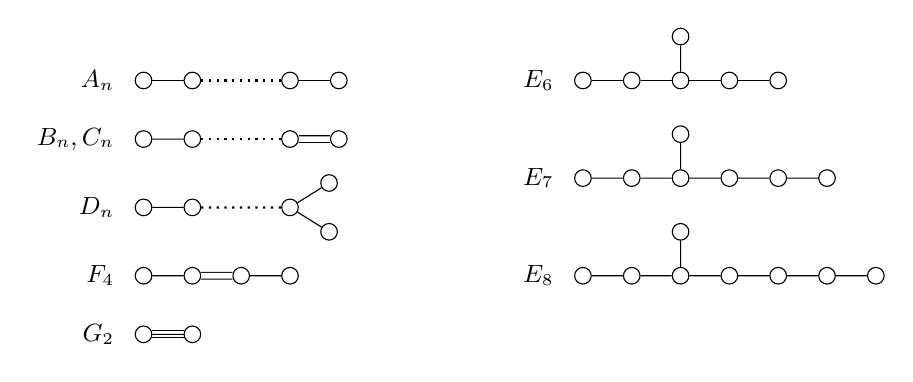
\begin{tikzpicture}[scale=0.62, every node/.style={font=\small}]
  % A_n
  \node[anchor=east] at (-0.4,0) {$A_n$};
  \foreach \i in {0,1,3,4} \node[L04bv] (A\i) at (\i,0) {};
  \draw (A0)--(A1); \draw[dotted,thick] (A1)--(A3); \draw (A3)--(A4);
  % B_n / C_n
  \node[anchor=east] at (-0.4,-1.2) {$B_n,C_n$};
  \foreach \i in {0,1,3,4} \node[L04bv] (B\i) at (\i,-1.2) {};
  \draw (B0)--(B1); \draw[dotted,thick] (B1)--(B3); \draw[L04bdbl] (B3)--(B4);
  % D_n
  \node[anchor=east] at (-0.4,-2.6) {$D_n$};
  \foreach \i in {0,1,3} \node[L04bv] (D\i) at (\i,-2.6) {};
  \node[L04bv] (Du) at (3.8,-2.1) {}; \node[L04bv] (Dd) at (3.8,-3.1) {};
  \draw (D0)--(D1); \draw[dotted,thick] (D1)--(D3); \draw (D3)--(Du); \draw (D3)--(Dd);
  % F4, G2
  \node[anchor=east] at (-0.4,-4.0) {$F_4$};
  \foreach \i in {0,1,2,3} \node[L04bv] (F\i) at (\i,-4.0) {};
  \draw (F0)--(F1); \draw[L04bdbl] (F1)--(F2); \draw (F2)--(F3);
  \node[anchor=east] at (-0.4,-5.2) {$G_2$};
  \node[L04bv] (G0) at (0,-5.2) {}; \node[L04bv] (G1) at (1,-5.2) {};
  \draw (G0)--(G1); \draw ([yshift=2pt]G0.east)--([yshift=2pt]G1.west);
  \draw ([yshift=-2pt]G0.east)--([yshift=-2pt]G1.west);
  % E6, E7, E8
  \begin{scope}[xshift=9cm]
  \foreach \n/\k/\y in {E_6/5/0, E_7/6/-2, E_8/7/-4} {
    \node[anchor=east] at (-0.4,\y) {$\n$};
    \foreach \i in {1,...,\k} \node[L04bv] (e\i) at (\i-1,\y) {};
    \foreach \i [evaluate=\i as \j using int(\i-1)] in {2,...,\k} \draw (e\i)--(e\j);
    \node[L04bv] (top) at (2,\y+0.9) {}; \draw (e3)--(top);
  }
  \end{scope}
\end{tikzpicture}
\end{center}
\end{addedblock}

\begin{remark}
It remains to show that each of
$A_n$, $B_n$, $C_n$, $D_n$, $E_6$, $E_7$, $E_8$, $F_4$, $G_2$ actually exists, i.e.\ to construct
the corresponding root systems. This is done in the next lecture; $G_2$ is left as an exercise
\added{(its $12$ roots were drawn in Lecture~4: check axioms 1)--4) directly)}.
\orig{p.~31: ``Existence of $A_n,\dots,F_4$: construct next time; $G_2$ -- ex.''}
\end{remark}

% ============================================================
\chapter{Lecture 6: Root systems and root lattices}
\label{L04b:ch:lecture6}

\section{Construction of crystallographic root systems}
\label{L04b:sec:construction}

\subsection*{\texorpdfstring{$A_n$}{An}}
In $A_n$ the simple roots are pairwise orthogonal or at angle $2\pi/3$.

Consider $x\in\Z^{n+1}$ such that $\sum_{i=1}^{n+1} x_i = 0$. These form an $n$-dimensional
\added{sublattice} $S$ of $\Z^{n+1}$. Let
\[
  \Delta = \{x\in S : \norm{x}=\sqrt2\}.
\]
That is, all but two coordinates are $0$, one coordinate is $+1$ and one is $-1$: the vectors
are the permutations of $(1,-1,0,\dots,0)$, so $|\Delta| = n(n+1)$. Choose the simple roots
\[
  \alpha_i = e_i - e_{i+1},\qquad i=1,\dots,n,
\]
\orig{diagram labelled $e_{i+1}-e_i$}
with matrix of coordinates and Dynkin diagram
\[
  \begin{bmatrix} 1 & -1 & & & \\ & 1 & -1 & & \\ & & \ddots & \ddots & \\ & & & 1 & -1\end{bmatrix}
  \qquad
  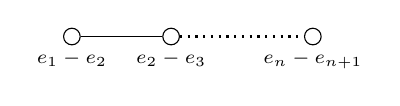
\begin{tikzpicture}[baseline=-3pt,scale=0.9]
    \foreach \x/\n/\l in {0/a/e_1-e_2,1.4/b/e_2-e_3,3.4/c/e_n-e_{n+1}}
      {\node[L04bv] (\n) at (\x,0) {}; \node[L04blab,below=2pt] at (\x,0) {$\l$};}
    \draw (a)--(b); \draw[dotted,thick] (b)--(c);
  \end{tikzpicture}
\]
To check the Dynkin diagram: the number of edges joining $\alpha_i$ and $\alpha_j$ is
$4\ip{\alpha_i}{\alpha_j}^2/(\norm{\alpha_i}^2\norm{\alpha_j}^2) = \ip{\alpha_i}{\alpha_j}^2\in\{1,0\}$,
and it is $1$ exactly when $j=i\pm1$.

Note that these roots generate the full sublattice $\{x\in\Z^{n+1}: \sum x_i=0\}$
\added{(any such $x$ equals $\sum_{k=1}^{n} (x_1+\dots+x_k)\,\alpha_k$)}. So the $A_n$ root lattice
is all of $S$. This description is maybe not so useful for visualizing, since $S$ sits inside
$\R^{n+1}$.

\begin{example}[$A_2$]
Simple roots $(-1,1,0)$ and $(0,-1,1)$, whose sum is $(-1,0,1)$; together with the negatives
$(1,-1,0)$, $(0,1,-1)$, $(1,0,-1)$ these are the six roots, lying in the plane
$x_1+x_2+x_3=0$. In that plane they form the familiar hexagonal configuration:
\begin{center}
\begin{tikzpicture}[scale=1.1]
  \foreach \a in {0,60,...,300} \draw[-{Stealth}] (0,0)--(\a:1);
  \draw[-{Stealth},very thick,addcol] (0,0)--(0:1) node[right,font=\scriptsize] {$\alpha_1$};
  \draw[-{Stealth},very thick,addcol] (0,0)--(120:1) node[above left,font=\scriptsize] {$\alpha_2$};
\end{tikzpicture}
\end{center}
\orig{p.~33: pink star in the plane $\sum x_i=0$}
\end{example}

\begin{example}[$A_3$]
The $12$ roots of $A_3$ are the $12$ nearest neighbours of the origin in the FCC lattice
(``the FCC system'') \added{--- the $A_3$ root lattice is the face-centred cubic lattice, with
kissing number $12$}.
\end{example}

\subsection*{\texorpdfstring{$B_n$}{Bn}}
$\Delta$ is the set of all integer vectors $x\in\Z^n$ of norm $1$ or norm $\sqrt2$, i.e.\
$\pm e_i$ and $\pm e_i\pm e_j$. So $|\Delta| = 2n + 4\binom n2 = 2n^2$. Simple roots:
\[
  \alpha_i = e_i - e_{i+1}\ (1\le i\le n-1),\qquad \text{short root } \alpha_n = e_n,
\]
\[
  \begin{bmatrix} 1 & -1 & & & \\ & 1 & -1 & & \\ & & \ddots & \ddots & \\ & & & 1 & -1\\ & & & & 1\end{bmatrix}
  \qquad
  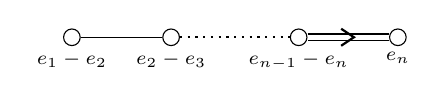
\begin{tikzpicture}[baseline=-3pt,scale=0.9]
    \foreach \x/\n/\l in {0/a/e_1-e_2,1.4/b/e_2-e_3,3.2/c/e_{n-1}-e_n,4.6/d/e_n}
      {\node[L04bv] (\n) at (\x,0) {}; \node[L04blab,below=2pt] at (\x,0) {$\l$};}
    \draw (a)--(b); \draw[dotted,thick] (b)--(c); \draw[L04bdbl] (c)--(d);
    \draw[thick] (3.8,0.12)--(3.98,0)--(3.8,-0.12);
  \end{tikzpicture}
\]
Sadly, from this construction the associated root lattice is all of $\Z^n$ \added{(it contains
every $e_i$)}, so we get nothing new.

\subsection*{\texorpdfstring{$C_n$}{Cn}}
$\Delta$ is the set of all integer vectors of the form $2x$ with $x\in\Z^n$ of length $1$, or
$x\in\Z^n$ of length $\sqrt2$; i.e.\ $\pm 2e_i$ and $\pm e_i\pm e_j$. Again
$|\Delta| = 2n + 4\binom n2 = 2n^2$. Simple roots:
\[
  \alpha_i = e_i - e_{i+1}\ (1\le i\le n-1),\qquad \text{long root } \alpha_n = 2e_n,
\]
\[
  \begin{bmatrix} 1 & -1 & & & \\ & 1 & -1 & & \\ & & \ddots & \ddots & \\ & & & 1 & -1\\ & & & & 2\end{bmatrix}
  \qquad
  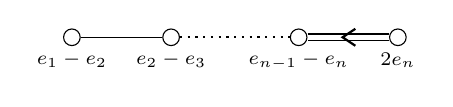
\begin{tikzpicture}[baseline=-3pt,scale=0.9]
    \foreach \x/\n/\l in {0/a/e_1-e_2,1.4/b/e_2-e_3,3.2/c/e_{n-1}-e_n,4.6/d/2e_n}
      {\node[L04bv] (\n) at (\x,0) {}; \node[L04blab,below=2pt] at (\x,0) {$\l$};}
    \draw (a)--(b); \draw[dotted,thick] (b)--(c); \draw[L04bdbl] (c)--(d);
    \draw[thick] (4.0,0.12)--(3.82,0)--(4.0,-0.12);
  \end{tikzpicture}
\]
\fixed{diagram drawn with a single last edge}
So the $C_n$ root lattice is the set of all integer vectors with \emph{even} coordinate sum.

\begin{example}[$B_2$ and $C_2$]
The two root systems, with the simple roots highlighted:
\begin{center}
\begin{tikzpicture}[scale=0.9]
  \foreach \v in {(1,0),(0,1),(-1,0),(0,-1),(1,1),(1,-1),(-1,1),(-1,-1)} \draw[-{Stealth},gray] (0,0)--\v;
  \draw[-{Stealth},very thick,addcol] (0,0)--(1,-1) node[below right,font=\scriptsize] {$\alpha_1=e_1-e_2$};
  \draw[-{Stealth},very thick,addcol] (0,0)--(0,1) node[above,font=\scriptsize] {$\alpha_2=e_2$};
  \node at (0,-1.7) {$B_2$};
  \begin{scope}[xshift=5cm]
  \foreach \v in {(2,0),(0,2),(-2,0),(0,-2),(1,1),(1,-1),(-1,1),(-1,-1)} \draw[-{Stealth},gray] (0,0)--\v;
  \draw[-{Stealth},very thick,addcol] (0,0)--(1,-1) node[below right,font=\scriptsize] {$\alpha_1=e_1-e_2$};
  \draw[-{Stealth},very thick,addcol] (0,0)--(0,2) node[above,font=\scriptsize] {$\alpha_2=2e_2$};
  \node at (0,-2.4) {$C_2$};
  \end{scope}
\end{tikzpicture}
\end{center}
\orig{redrawn; sketch showed only $\alpha_1,\alpha_2$}
\added{In both, the simple roots meet at angle $3\pi/4$; $C_2$ is $B_2$ rotated by $\pi/4$ and rescaled.}
\end{example}

\subsection*{\texorpdfstring{$D_n$}{Dn}}
$\Delta$ is the set of all integer vectors $x\in\Z^n$ of length $\sqrt2$, i.e.\ $\pm e_i\pm e_j$, so
\[
  |\Delta| = 4\binom n2 = 2n(n-1).
\]
\fixed{notes: $2\binom n2$}
Simple roots:
\[
  \alpha_i = e_i - e_{i+1}\ (1\le i\le n-1)\qquad\text{and}\qquad \alpha_n = e_{n-1}+e_n,
\]
\[
  \begin{bmatrix} 1 & -1 & & & \\ & \ddots & \ddots & & \\ & & 1 & -1 & \\ & & & 1 & -1\\ & & & 1 & 1\end{bmatrix}
  \qquad
  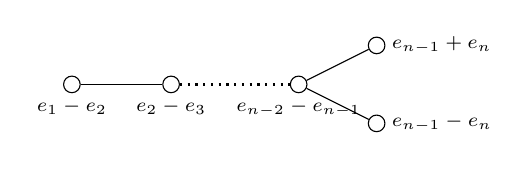
\begin{tikzpicture}[baseline=-3pt,scale=0.9]
    \foreach \x/\n/\l in {0/a/e_1-e_2,1.4/b/e_2-e_3,3.2/c/e_{n-2}-e_{n-1}}
      {\node[L04bv] (\n) at (\x,0) {}; \node[L04blab,below=2pt] at (\x,0) {$\l$};}
    \node[L04bv] (u) at (4.3,0.55) {}; \node[L04blab,right=2pt] at (4.3,0.55) {$e_{n-1}+e_n$};
    \node[L04bv] (d) at (4.3,-0.55) {}; \node[L04blab,right=2pt] at (4.3,-0.55) {$e_{n-1}-e_n$};
    \draw (a)--(b); \draw[dotted,thick] (b)--(c); \draw (c)--(u); \draw (c)--(d);
  \end{tikzpicture}
\]
This also generates the lattice $\{x\in\Z^n : \text{the coordinate sum is even}\}$, the same as
for $C_n$. (I can't draw $D_4$, sadly.)

\subsection*{\texorpdfstring{$F_4$}{F4}}
$\Delta$ is the set of vectors $x\in\R^4$ of length $1$ or $\sqrt2$ such that the coordinates of
$2x$ are all even or all odd integers. \added{Explicitly: $\pm e_i$ ($8$), $\pm e_i\pm e_j$ ($24$) and
$\tfrac12(\pm1,\pm1,\pm1,\pm1)$ ($16$), so $|\Delta|=48$.} Simple roots:
\[
  \alpha_1 = (1,-1,0,0),\quad \alpha_2=(0,1,-1,0),\quad \alpha_3=(0,0,1,0),\quad
  \alpha_4 = -\tfrac12(1,1,1,1),
\]
\begin{center}
  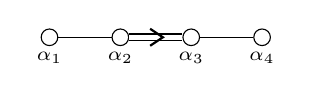
\begin{tikzpicture}[baseline=-3pt,scale=0.9]
    \foreach \x/\n in {0/1,1/2,2/3,3/4}
      {\node[L04bv] (f\n) at (\x,0) {}; \node[L04blab,below=2pt] at (\x,0) {$\alpha_\n$};}
    \draw (f1)--(f2); \draw[L04bdbl] (f2)--(f3); \draw (f3)--(f4);
    \draw[thick] (1.42,0.12)--(1.6,0)--(1.42,-0.12);
  \end{tikzpicture}
\end{center}
(check by hand). \added{Indeed $\ip{\alpha_1}{\alpha_2}=-1$ with both of length $\sqrt2$ (angle $2\pi/3$);
$\ip{\alpha_2}{\alpha_3}=-1$ with lengths $\sqrt2,1$ (angle $3\pi/4$, double edge);
$\ip{\alpha_3}{\alpha_4}=-\frac12$ with both of length $1$ (angle $2\pi/3$); all other pairs are orthogonal.}

The $F_4$ root lattice: all coordinates are integers, or all coordinates are halves of odd integers
--- no mixing. \added{That is, $\Z^4\cup(\Z^4+\tfrac12(1,1,1,1))$, which is $D_4^*$, a scaled copy of $D_4$.}

\subsection*{\texorpdfstring{$G_2$}{G2}}
We already drew this one (the $12$ roots form a ``star of David'', two hexagons of lengths $1$ and
$\sqrt3$). \orig{star sketch, see Lecture~4}
The $G_2$ root lattice coincides with the $A_2$ root lattice \added{(the hexagonal lattice)}.

% ------------------------------------------------------------
\section{The \texorpdfstring{$E_8$}{E8} root system}
\label{L04b:sec:E8}

\begin{definition}\label{L04b:def:E8}
The $E_8$ root system consists of the $|\Delta| = 240$ vectors in $\R^8$ of the forms
\[
  \pm e_i \pm e_j\ (i\neq j) \qquad\text{and}\qquad \tfrac12(\pm e_1 \pm \dots \pm e_8)
  \ \added{\text{with an even number of minus signs}}.
\]
\fixed{added the even-sign condition}
\added{There are $4\binom82=112$ of the first kind and $2^7=128$ of the second.}
\end{definition}

Simple roots:
\[
  \alpha_i = e_i-e_{i+1}\ (1\le i\le 6),\qquad \alpha_7 = e_6+e_7,\qquad \alpha_8 = -\tfrac12(1,\dots,1),
\]
\[
  \begin{bmatrix}
   1&-1&0&0&0&0&0&0\\ &1&-1&0&0&0&0&0\\ &&1&-1&0&0&0&0\\ &&&1&-1&0&0&0\\ &&&&1&-1&0&0\\
   &&&&&1&-1&0\\ &&&&&1&1&0\\ -\frac12&-\frac12&-\frac12&-\frac12&-\frac12&-\frac12&-\frac12&-\frac12
  \end{bmatrix}
  \qquad
  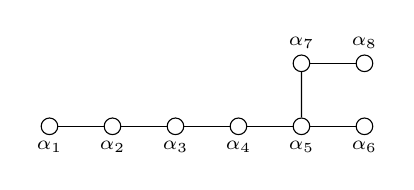
\begin{tikzpicture}[baseline=-3pt,scale=0.8]
    \foreach \i in {1,...,6} {\node[L04bv] (g\i) at (\i-1,0) {}; \node[L04blab,below=2pt] at (\i-1,0) {$\alpha_{\i}$};}
    \node[L04bv] (g7) at (4,1) {}; \node[L04blab,above=2pt] at (4,1) {$\alpha_7$};
    \node[L04bv] (g8) at (5,1) {}; \node[L04blab,above=2pt] at (5,1) {$\alpha_8$};
    \foreach \i/\j in {1/2,2/3,3/4,4/5,5/6,5/7,7/8} \draw (g\i)--(g\j);
  \end{tikzpicture}
\]
\added{(Check: $\ip{\alpha_7}{\alpha_5}=-1$, $\ip{\alpha_7}{\alpha_6}=0$, $\ip{\alpha_8}{\alpha_7}=-1$ and
$\ip{\alpha_8}{\alpha_i}=0$ for $i\le 6$; the arms at $\alpha_5$ give $(p,q,r)=(5,3,2)$.)}

This generates the lattice $E_8$ of all $x\in\R^8$ such that
\begin{enumerate}[label=\arabic*)]
  \item the coordinates are all integers or all half-integers \added{(halves of odd integers)}, and
  \item the sum of the coordinates is even.
\end{enumerate}

This is clearly related to $D_8$. Consider the ``deep holes'' of the $D_n$ lattice, i.e.\ the
half-integer points such as $h=\frac12(1,\dots,1)$. In dimension $8$,
\[
  \norm{\tfrac12(1,\dots,1)} = \sqrt2,
\]
and a typical shortest lattice vector has $\norm{(1,1,0,\dots,0)}=\sqrt2$. Similarly,
\[
  \norm{(1,1,0,\dots,0)-\tfrac12(1,\dots,1)} = \sqrt2 .
\]
So if we have $D_8$, there is another copy $D_8+h$ that fits into the holes of $D_8$ without
decreasing the minimal distance: $E_8 = D_8\cup(D_8+h)$.
\added{(For general $n$, $h$ is at distance $\sqrt n/2$ from $D_n$; this equals the minimal
distance $\sqrt2$ exactly when $n=8$.)}

\subsection*{\texorpdfstring{$E_7$, $E_6$}{E7, E6}}
Let $v=(1,1,\dots,1)$ and $w=-e_7-e_8$. Then
\[
  E_7 = E_8\cap v^\perp,\qquad E_6 = E_8\cap \langle w,v\rangle^\perp .
\]
\added{Here $\frac12 v=-\alpha_8$ and $w$ are roots with $\ip{\tfrac12 v}{w}=-1$, so they span an
$A_2$; thus $E_7$ and $E_6$ are the orthogonal complements of an $A_1$ and an $A_2$ in $E_8$.}

These descriptions are not so satisfying, but perhaps there is an easy-to-see construction given
by collapsing simple chains: replace $\alpha_1,\alpha_2$ by $\alpha_1+\alpha_2$, then
$\alpha_1+\alpha_2,\alpha_3$ by $\alpha_1+\alpha_2+\alpha_3$, and so on.
\begin{center}
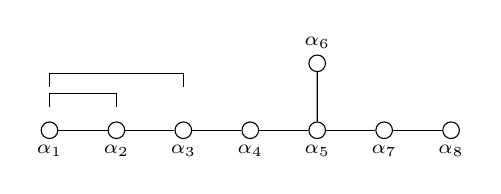
\begin{tikzpicture}[scale=0.85]
  \foreach \x/\n in {0/1,1/2,2/3,3/4,4/5,5/7,6/8}
    {\node[L04bv] (h\n) at (\x,0) {}; \node[L04blab,below=2pt] at (\x,0) {$\alpha_\n$};}
  \node[L04bv] (h6) at (4,1) {}; \node[L04blab,above=2pt] at (4,1) {$\alpha_6$};
  \foreach \i/\j in {1/2,2/3,3/4,4/5,5/7,7/8,5/6} \draw (h\i)--(h\j);
  \draw (0,0.35)--(0,0.55)--(1,0.55)--(1,0.35);
  \draw (0,0.65)--(0,0.85)--(2,0.85)--(2,0.65);
\end{tikzpicture}
\end{center}
By the collapsing lemma, $\alpha_1+\alpha_2,\alpha_3,\dots,\alpha_8$ is a simple system of type $E_7$,
and $\alpha_1+\alpha_2+\alpha_3,\alpha_4,\dots,\alpha_8$ one of type $E_6$, \added{so the lattices they
generate are copies of the $E_7$, $E_6$ root lattices inside $E_8$.} This continues
\added{(collapsing suitable chains)} to
\[
  D_5,\quad D_4,\quad A_3,\quad A_2,\quad A_1 .
\]

\begin{exercise}
Find other constructions of $E_8$. \added{(For instance via the extended Hamming code and
Construction~A, \S\ref{L04b:sec:codes}.)}
\end{exercise}

% ------------------------------------------------------------
\section{Laminated lattices}
\label{L04b:sec:laminated}

Before (Lecture~4) we had the lattices
\[
  A_1,\ A_2,\ A_3,\ D_4,\ D_5,\ E_6,\ E_7,\ E_8
\]
as the best lattice packings, and best known packings, in dimensions $1$ to $8$. Somehow these
are all related to $E_8$ (as we just saw, they all sit inside $E_8$).

\begin{addedblock}
Optimality among lattices is proven in dimensions $1$--$8$ (Lagrange $n=2$, Gauss $n=3$,
Korkine--Zolotarev $n=4,5$, Blichfeldt $n=6,7,8$); among \emph{all} packings it is proven for
$n=2$ (Thue, Fejes T\'oth), $n=3$ (Hales) and $n=8$ (Viazovska, posted March 2016, during this course).
Similarly the Leech lattice is optimal in dimension $24$ (Cohn--Kumar among lattices;
Cohn--Kumar--Miller--Radchenko--Viazovska 2016/17 among all packings).
\end{addedblock}

Dimension $9$ is, as far as I know, still unknown.
\added{(This is still the case, to the editor's knowledge.)}

The best constructions for lattices come from an ``inductive'' process. Start with the even
integers $\Lambda_1 = 2\Z\subset\R^1$.

\begin{definition}\label{L04b:def:laminated}
The \emph{$n$-dimensional laminated lattice} $\Lambda_n$ is a lattice of maximal density among
all lattices in $\R^n$ with shortest vector of length $\norm{x}=2$ that contain $\Lambda_{n-1}$
as a sublattice.
\end{definition}
So $\Lambda_n$ is obtained by gluing: $\Lambda_n=\langle \Lambda_{n-1}, g\rangle$\added{, i.e.\ by stacking
layers $\Lambda_{n-1}+kg$, $k\in\Z$, with each new layer placed over the deepest holes of the previous one}.
\begin{center}
\begin{tikzpicture}[scale=0.45]
  % A1
  \foreach \i in {0,...,4} \fill (\i,0) circle (2.5pt);
  \node at (2,-1.6) {$A_1$};
  \draw[-{Stealth}] (5,0)--(6.5,0);
  % A2
  \begin{scope}[xshift=7.5cm]
    \foreach \j in {-2,...,2} \foreach \i in {0,...,4} {
      \pgfmathsetmacro{\xx}{\i+0.5*mod(abs(\j),2)} \fill (\xx,{0.866*\j}) circle (2.5pt); }
    \node at (2.2,-3.0) {$A_2$};
  \end{scope}
  \draw[-{Stealth}] (13.3,0)--(14.8,0);
  % A3: hexagonal layer + next layer over holes
  \begin{scope}[xshift=16cm]
    \foreach \j in {-2,...,2} \foreach \i in {0,...,4} {
      \pgfmathsetmacro{\xx}{\i+0.5*mod(abs(\j),2)} \fill (\xx,{0.866*\j}) circle (2.5pt); }
    \foreach \j in {-2,...,1} \foreach \i in {0,...,3} {
      \pgfmathsetmacro{\xx}{\i+0.5+0.5*mod(abs(\j),2)} \draw (\xx,{0.866*\j+0.2887}) circle (3.5pt); }
    \node at (2.2,-3.0) {$A_3$};
  \end{scope}
  \draw[-{Stealth}] (21.8,0)--(23.3,0);
  \node at (24.6,0) {$\cdots\ E_8$};
\end{tikzpicture}
\end{center}
\orig{p.~40 sketch; circles = next layer}
The laminated lattices $\Lambda_1,\dots,\Lambda_8$ coincide with the root lattices above
\added{(scaled to minimal length $2$)}.

\begin{remark}
Dimension $9$ is unusual: there is a continuous family of packings built from layers of $\Lambda_8$,
\fixed{notes: ``cts family of lattices''}
all of the same density as $\Lambda_9$. \added{These are the ``fluid'' packings; in general they are
\emph{not} lattice packings, so ``family of lattices'' should be read as ``family of packings'' (see
Conway--Sloane, \emph{Sphere Packings, Lattices and Groups}, Ch.~1 and Ch.~6).}
\end{remark}

% ------------------------------------------------------------
\section{Dimension 10: codes and Construction A}
\label{L04b:sec:codes}

In dimension $10$, a \emph{non-lattice} packing beats the best known lattices.

\begin{definition}\label{L04b:def:code}
A \emph{binary code} of length $n$ is a subset $C\subseteq\{0,1\}^n$ of the binary words of length $n$.
The elements of $C$ are the \emph{code words}. \added{The \emph{Hamming distance} between two words is the
number of positions in which they differ; $d(C)$ denotes the minimal distance between distinct code words.}
\end{definition}

\begin{definition}[Construction A]\label{L04b:def:constrA}
Given a binary code $C$ of length $n$, there is a packing
\fixed{notes: $|C|=n$}
\[
  P(C) = \{x\in\Z^n : x \bmod 2 \in C\}.
\]
\end{definition}
\begin{addedblock}
Two distinct points of $P(C)$ either differ by an element of $2\Z^n$ (distance $\ge2$) or reduce to
different code words, hence differ by $\pm1$ in at least $d(C)$ coordinates (distance $\ge\sqrt{d(C)}$).
So $P(C)$ is a packing of balls of radius $\frac12\min(2,\sqrt{d(C)})$ with $|C|$ centres per cube
$[0,2)^n$, and its centre density is $|C|\,2^{-n}\big(\tfrac12\min(2,\sqrt{d(C)})\big)^n$.
\end{addedblock}

This gives some relation between packing problems in high dimensions and error detecting /
error correcting codes. Think of a code word sent through a continuous channel and received
with an error of size up to $\varepsilon$: the centres of the $\varepsilon$-spheres of a packing correspond
to code words that are at distance $\ge 2\varepsilon$ apart. Dense packings correspond to large collections of
code words that are well separated.
\orig{sketch: $\varepsilon$-ball around a code word}

\begin{example}[Block codes]
The $(6,3)$ repetition code repeats the pattern: $101\mapsto101101$. The $(3,2)$ parity check code
(mod $2$) appends a parity bit: $11\mapsto 110$. We can see the latter on the Hamming cube: its code
words $000,011,101,110$ all have Hamming distance $2$, i.e.\ are $2$ bits apart.
\begin{center}
\begin{tikzpicture}[scale=1.3]
  \coordinate (000) at (0,0); \coordinate (100) at (1,0); \coordinate (010) at (0.45,0.35);
  \coordinate (001) at (0,1); \coordinate (110) at (1.45,0.35); \coordinate (101) at (1,1);
  \coordinate (011) at (0.45,1.35); \coordinate (111) at (1.45,1.35);
  \draw (000)--(100)--(101)--(001)--cycle; \draw (001)--(011)--(111)--(101); \draw (100)--(110)--(111);
  \draw[dashed] (000)--(010)--(110); \draw[dashed] (010)--(011);
  \foreach \p in {000,011,101,110} {\fill[addcol] (\p) circle (2.2pt);}
  \node[below left,font=\scriptsize] at (000) {$000$}; \node[above,font=\scriptsize] at (011) {$011$};
  \node[right,font=\scriptsize] at (101) {$101$}; \node[right,font=\scriptsize] at (110) {$110$};
\end{tikzpicture}
\end{center}
In general, parity check codes (all even-weight words) correspond to $D_n$, the lattice with even
coordinate sums.
\end{example}

Construction A thus links binary codes and lattices: $P(C)$ is a lattice if and only if $C$ is a
\emph{linear} code, that is, sums of code words (mod $2$) are code words.
The Hamming codes give $E_7$ and $E_8$. \added{More precisely (after scaling by $1/\sqrt2$): the extended
Hamming code $[8,4,4]$ gives $E_8$ ($16+14\cdot16=240$ vectors of norm $4$ in $P(C)$), and the $[7,3,4]$
simplex code, the dual of the Hamming code $[7,4,3]$, gives $E_7$ ($14+7\cdot16=126$).}

\subsection*{The code \texorpdfstring{$C_{10}$}{C10}}
So in dimension $10$ there is a special binary code $C_{10}$ \added{(Best's code)}, which is unique
\added{(Litsyn--Vardy)} and quite dense. It is based on a Gray code, or reflected binary code.

\begin{definition}
A \emph{Gray code} is a map $(\Z_2)^n\to(\Z_2)^n$, \added{a re-ordering of all binary words of length $n$},
where the successor of an element differs by a single bit flip.
\end{definition}
\[
  \begin{array}{ccc}
    \text{binary} & & \text{Gray}\\ \hline
    00 & 0 & 00\\ 01 & 1 & 01\\ 10 & 2 & 11\\ 11 & 3 & 10
  \end{array}
\]
There is a replacement procedure to convert between binary and Gray codes.

\begin{exercise}
Find the conversion binary $\leftrightarrow$ Gray, and iterate it to get the Gray code of length $n$.
\added{(Hint: $g = b \oplus (b\gg1)$; conversely $b_k = g_1\oplus\dots\oplus g_k$ from the leading bit.)}
\end{exercise}

In dimension $10$ \added{we look for} binary codes with minimum distance at least $4$. We construct
$C_{10}$ as follows. Take $(a,b,c,d,e)\in(\Z_4)^5$ satisfying
\[
  b,c,d\in\{\pm1\},\qquad a = c-d,\qquad e = b+c,
\]
\unclear{$\{\pm1\}$: a crossed-out entry; $\{\pm1\}$ fits the count $2^3$}
together with all cyclic permutations thereof. Then apply the Gray map
\[
  0\mapsto 00,\quad 1\mapsto 01,\quad 2\mapsto 11,\quad 3\mapsto 10.
\]
This gives $8\cdot5=40$ code words ($2^3$ choices of $(b,c,d)$ times $5$ cyclic shifts) of length $10$.

\begin{claim}
The Hamming distance between distinct code words of $C_{10}$ is at least $4$.
\end{claim}
\begin{addedblock}
The Gray map is an isometry from $\Z_4$ with the Lee metric ($d(0,2)=d(1,3)=2$, other distinct pairs
distance $1$) to $\Z_2^2$ with the Hamming metric, so it suffices to check Lee distance $\ge4$ in $(\Z_4)^5$.
(Editor: confirmed by direct computer check of all $\binom{40}{2}$ pairs; the $40$ words are distinct.)
\end{addedblock}

Moreover $A(10,4)=40$, i.e.\ $40$ is the maximal size of a binary code of length $10$ and minimal
distance $4$, so $C_{10}$ is optimal for dimension $10$.
\unclear{notes: ``LP bound $\Rightarrow<40.\ldots$''; $A(10,4)=40$ is due to Best (c.~1980)}
\begin{addedblock}
Construction A applied to $C_{10}$ gives the non-lattice packing $P_{10c}$: radius $1$ and $40$ centres
per $2^{10}$ volume, so centre density $40/2^{10}=5/128\approx0.0391$, larger than that of the best known
lattice $\Lambda_{10}$ (centre density $1/(16\sqrt3)\approx0.0361$). See Conway--Sloane, Ch.~5.
\end{addedblock}

% ------------------------------------------------------------
\section{An aside: lattice vs.\ non-lattice packings of other objects}
\label{L04b:sec:aside}

For other objects than balls, the question of lattice versus non-lattice packings looks different:
\begin{itemize}
  \item ellipsoid packings;
  \item polygon packings;
  \item honeycomb (HCB) and bubble problems. \unclear{``HCB'', ``Bubble prob.''?}
\end{itemize}
\added{For example, in the plane a lattice packing is optimal for any centrally symmetric convex body
(Fejes T\'oth, Rogers), but not for some non-symmetric ones; and congruent ellipsoids in $\R^3$ can be packed
more densely by non-lattice arrangements than by any lattice (Bezdek--Kuperberg). Hales proved the honeycomb
conjecture in 1999.} Density issues are subtle here, e.g.\ in $2$d versus $1$d.

On the same page there is a computation: with $a^2b=1$,
\[
  \begin{bmatrix} 1&&\\ &a&\\ &&a^2\end{bmatrix}
  \begin{pmatrix}1\\1\\1\end{pmatrix} = \begin{pmatrix}1\\a\\a^2\end{pmatrix},\qquad
  \begin{bmatrix} 1&&\\ &a&\\ &&a^2\end{bmatrix}
  \begin{pmatrix}a\\a\\b\end{pmatrix} = \begin{pmatrix}a\\a^2\\1\end{pmatrix}.
\]
\unclear{purpose unclear; maybe an ellipsoid-packing example}

% ------------------------------------------------------------
\section*{Projects and quiz}
\orig{admin (date, room) omitted}
Ideas for projects:
\begin{itemize}
  \item error correcting codes and information theory;
  \item other sphere packing bounds;
  \item entropy of jammed systems;
  \item translation of an older work on packings. \unclear{last item barely legible}
\end{itemize}
Format of the quiz: definitions, short answers, sketches.
